% Capitolul 7: Cointegrare și Modele VECM
% Prezentare academică de calitate Harvard
% Program de licență, Academia de Studii Economice din București

\documentclass[9pt, aspectratio=169, t]{beamer}

% Asigură încadrarea conținutului pe diapozitive
\setbeamersize{text margin left=8mm, text margin right=8mm}

%=============================================================================
% CONFIGURARE TEMĂ ȘI STIL
%=============================================================================
\usetheme{default}
% Using default theme for clean header/footer control

% Color Palette (matching Redispatch PDF)
\definecolor{MainBlue}{RGB}{26, 58, 110}
\definecolor{AccentBlue}{RGB}{26, 58, 110}
\definecolor{IDAred}{RGB}{205, 0, 0}
\definecolor{DarkGray}{RGB}{51, 51, 51}
\definecolor{MediumGray}{RGB}{128, 128, 128}
\definecolor{LightGray}{RGB}{248, 248, 248}
\definecolor{VeryLightGray}{RGB}{235, 235, 235}
\definecolor{KeynoteGray}{RGB}{218, 218, 218}
\definecolor{SectionGray}{RGB}{120, 120, 120}
\definecolor{FooterGray}{RGB}{100, 100, 100}
\definecolor{Crimson}{RGB}{220, 53, 69}
\definecolor{Forest}{RGB}{46, 125, 50}
\definecolor{Amber}{RGB}{181, 133, 63}
\definecolor{Orange}{RGB}{230, 126, 34}
\definecolor{Purple}{RGB}{142, 68, 173}

% Gradient background (exact Keynote 315° gradient: white to RGB 218,218,218)
\setbeamertemplate{background}{%
    \begin{tikzpicture}[remember picture, overlay]
        \shade[shading=axis, shading angle=315,
        top color=white, bottom color=KeynoteGray]
        (current page.south west) rectangle (current page.north east);
    \end{tikzpicture}%
}
% Fallback solid color for compatibility
\setbeamercolor{background canvas}{bg=}

\setbeamercolor{palette primary}{bg=MainBlue, fg=white}
\setbeamercolor{palette secondary}{bg=MainBlue!85, fg=white}
\setbeamercolor{palette tertiary}{bg=MainBlue!70, fg=white}
\setbeamercolor{structure}{fg=MainBlue}
\setbeamercolor{title}{fg=IDAred}
\setbeamercolor{frametitle}{fg=IDAred, bg=}
\setbeamercolor{block title}{bg=MainBlue, fg=white}
\setbeamercolor{block body}{bg=VeryLightGray, fg=DarkGray}
\setbeamercolor{block title alerted}{bg=Crimson, fg=white}
\setbeamercolor{block body alerted}{bg=Crimson!8, fg=DarkGray}
\setbeamercolor{block title example}{bg=Forest, fg=white}
\setbeamercolor{block body example}{bg=Forest!8, fg=DarkGray}
\setbeamercolor{item}{fg=MainBlue}

% Footer colors (override Madrid theme blue)
\setbeamercolor{author in head/foot}{fg=FooterGray, bg=}
\setbeamercolor{title in head/foot}{fg=FooterGray, bg=}
\setbeamercolor{date in head/foot}{fg=FooterGray, bg=}
\setbeamercolor{section in head/foot}{fg=FooterGray, bg=}
\setbeamercolor{subsection in head/foot}{fg=FooterGray, bg=}

% Bullet styles (apply everywhere including blocks)
\setbeamertemplate{itemize item}{\color{MainBlue}$\boxdot$}
\setbeamertemplate{itemize subitem}{\color{MainBlue}$\blacktriangleright$}
\setbeamertemplate{itemize subsubitem}{\color{MainBlue}\tiny$\bullet$}
\setbeamertemplate{itemize/enumerate body begin}{\normalsize}
\setbeamertemplate{itemize/enumerate subbody begin}{\normalsize}

% Item spacing - compact style
\setlength{\leftmargini}{10pt}       % Level 1: minimal indent
\setlength{\leftmarginii}{10pt}      % Level 2: minimal additional indent
% Compact list spacing (zero extra space before/after lists in blocks)
\makeatletter
\def\@listi{\leftmargin\leftmargini \topsep 0pt \parsep 0pt \itemsep 0pt}
\def\@listii{\leftmargin\leftmarginii \topsep 0pt \parsep 0pt \itemsep 0pt}
\makeatother

\setbeamertemplate{navigation symbols}{}

%=============================================================================
% CUSTOM HEADLINE
%=============================================================================
\setbeamertemplate{headline}{%
    \vskip10pt%
    \hbox to \paperwidth{%
        \hskip0.5cm%
        {\small\color{FooterGray}\renewcommand{\hyperlink}[2]{##2}\insertsectionhead}%
        \hfill%
        \textcolor{FooterGray}{\small\insertframenumber}%
        \hskip0.5cm%
    }%
    \vskip4pt%
    {\color{FooterGray}\hrule height 0.4pt}%
}

%=============================================================================
% CUSTOM FOOTER
%=============================================================================
\usepackage{fontawesome5}

\setbeamertemplate{footline}{%
    {\color{FooterGray}\hrule height 0.4pt}%
    \vskip4pt%
    \hbox to \paperwidth{%
        \hskip0.5cm%
        \textcolor{FooterGray}{\small Analiza și Prognoza Seriilor de Timp}%
        \hfill%
        \raisebox{-0.1em}{%
            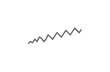
\begin{tikzpicture}[x=0.08em, y=0.08em, line width=0.4pt]
                \draw[FooterGray] (0,3) -- (1,4) -- (2,3.5) -- (3,5) -- (4,4) -- (5,6) -- (6,5.5) -- (7,4) -- (8,5) -- (9,7) -- (10,6) -- (11,5) -- (12,6.5) -- (13,8) -- (14,7) -- (15,6) -- (16,7.5) -- (17,9) -- (18,8) -- (19,7) -- (20,8.5) -- (21,10) -- (22,9) -- (23,8) -- (24,9.5);
            \end{tikzpicture}%
        }%
        \hskip0.5cm%
    }%
    \vskip6pt%
}

%=============================================================================
% PACHETE
%=============================================================================
\usepackage[utf8]{inputenc}
\usepackage[T1]{fontenc}
\usepackage{amsmath, amssymb, amsthm}
\usepackage{mathtools}
\usepackage{bm}
\usepackage{tikz}
\usetikzlibrary{arrows.meta, positioning, shapes, calc, decorations.pathreplacing, shadings}
\usepackage{booktabs}
\usepackage{multirow}
\usepackage{array}
\usepackage{graphicx}
\usepackage{hyperref}
\usepackage{colortbl}
\hypersetup{colorlinks=true, linkcolor=MainBlue, urlcolor=MainBlue}
\graphicspath{{../../logos/}{../../charts/}}
\hfuzz=2pt  % Suppress tiny overfull warnings (<2pt)

%=============================================================================
%=============================================================================
% Usage: \quantlet{QuantletName}{https://github.com/...}
\newcommand{\quantlet}[2]{%
    \hfill\href{#2}{\raisebox{-0.15em}{\includegraphics[height=0.7em]{ql_logo.png}}\textcolor{MainBlue}{\tiny\ #1}}%
}


%=============================================================================
% MEDII PENTRU TEOREME
%=============================================================================
\theoremstyle{definition}
\setbeamertemplate{theorems}[numbered]
\newtheorem{defn}{Definiție}
\newtheorem{thm}{Teoremă}
\newtheorem{prop}{Propoziție}
\newtheorem{rmk}{Observație}

%=============================================================================
% COMENZI PERSONALIZATE
%=============================================================================
\newcommand{\E}{\mathbb{E}}
\newcommand{\Var}{\text{Var}}
\newcommand{\Cov}{\text{Cov}}
\newcommand{\Corr}{\text{Corr}}
\newcommand{\R}{\mathbb{R}}
\newcommand{\N}{\mathbb{N}}
\newcommand{\Z}{\mathbb{Z}}
\newcommand{\RMSE}{\text{RMSE}}
\newcommand{\MAE}{\text{MAE}}
\newcommand{\MAPE}{\text{MAPE}}
\newcommand{\bY}{\mathbf{Y}}
\newcommand{\bA}{\mathbf{A}}
\newcommand{\bSigma}{\boldsymbol{\Sigma}}
\newcommand{\bPhi}{\boldsymbol{\Phi}}
\newcommand{\bGamma}{\boldsymbol{\Gamma}}
\newcommand{\bPi}{\boldsymbol{\Pi}}
\newcommand{\bc}{\mathbf{c}}
\newcommand{\balpha}{\boldsymbol{\alpha}}
\newcommand{\bbeta}{\boldsymbol{\beta}}
\newcommand{\bepsilon}{\boldsymbol{\varepsilon}}

%=============================================================================
% PAGINĂ TITLU PERSONALIZATĂ
%=============================================================================
\defbeamertemplate*{title page}{hybrid}[1][]
{
    \vspace{0.2cm}
    % Logos row - top header (with clickable links)
    \begin{center}
        \href{https://www.ase.ro}{\includegraphics[height=1.0cm]{ase_logo.png}}\hspace{0.3cm}%
        \href{https://theida.net}{\includegraphics[height=1.0cm]{ida_logo.png}}\hspace{0.3cm}%
        \href{https://blockchain-research-center.com}{\includegraphics[height=1.0cm]{brc_logo.png}}\hspace{0.3cm}%
        \href{https://www.ai4efin.ase.ro}{\includegraphics[height=1.0cm]{ai4efin_logo.png}}\hspace{0.3cm}%
        \href{https://ipe.ro/new}{\includegraphics[height=1.0cm]{acad_logo.png}}\hspace{0.3cm}%
        \href{https://www.digital-finance-msca.com}{\includegraphics[height=1.0cm]{msca_logo.png}}%
    \end{center}

    \vspace{0.6cm}

    % Main title with Q logos on sides (with clickable links)
    \begin{center}
        \begin{minipage}{0.1\textwidth}
            \centering
            \href{https://quantlet.com}{\includegraphics[height=1.1cm]{ql_logo.png}}
        \end{minipage}%
        \begin{minipage}{0.78\textwidth}
            \centering
            {\LARGE\bfseries\usebeamercolor[fg]{title}\inserttitle}

            \vspace{0.3cm}

            {\usebeamerfont{subtitle}\usebeamercolor[fg]{title}\insertsubtitle}
        \end{minipage}%
        \begin{minipage}{0.1\textwidth}
            \centering
            \href{https://quantinar.com}{\includegraphics[height=1.1cm]{qr_logo.png}}
        \end{minipage}
    \end{center}

    \vspace{0.6cm}

    % Authors (left aligned)
    \hspace{0.5cm}{\usebeamerfont{author}\insertauthor}

    \vspace{0.3cm}

    % Institute/Affiliations (left aligned)
    \hspace{0.5cm}\begin{minipage}[t]{0.9\textwidth}
        \raggedright\small\insertinstitute
    \end{minipage}
}

%=============================================================================
% INFORMAȚII TITLU
%=============================================================================
\title[Analiza Seriilor de Timp]{Analiza și Prognoza Seriilor de Timp}
\subtitle{Capitolul 7: Cointegrare și Modele VECM}
\author[D.T. Pele]{Daniel Traian PELE}
\institute{Academia de Studii Economice din București\\
IDA Institute Digital Assets\\
Blockchain Research Center\\
AI4EFin Artificial Intelligence for Energy Finance\\
Academia Română, Institutul de Prognoză Economică\\
MSCA Digital Finance}
\date{}

\begin{document}

% Title page (no header/footer)
{
\setbeamertemplate{headline}{}
\setbeamertemplate{footline}{}
\begin{frame}
    \titlepage
\end{frame}
}

%=============================================================================
% OUTLINE
%=============================================================================
\begin{frame}{Cuprins}
    \vspace{-0.3cm}
    {\small
    \begin{columns}[T]
        \begin{column}{0.48\textwidth}
            \begin{block}{Fundamente}
                \begin{itemize}\setlength{\itemsep}{3pt}
                    \item Motivație
                    \item Regresia Falsă
                    \item Conceptul de Cointegrare
                    \item Metoda Engle-Granger
                    \item Metoda Johansen
                \end{itemize}
            \end{block}
        \end{column}
        \begin{column}{0.48\textwidth}
            \begin{exampleblock}{Aplicații}
                \begin{itemize}\setlength{\itemsep}{3pt}
                    \item Estimarea VECM
                    \item Considerații Practice
                    \item Exemple Practice
                    \item Studiu de caz: Rate de dobândă
                    \item Rezumat și Quiz
                \end{itemize}
            \end{exampleblock}
        \end{column}
    \end{columns}
    }
\end{frame}

%=============================================================================
% LEARNING OBJECTIVES
%=============================================================================
\begin{frame}{Obiective de învățare}
    \begin{block}{La finalul acestui capitol, veți fi capabili să:}
        \begin{itemize}\setlength{\itemsep}{2pt}
            \item \textbf{Cointegrare}: Înțelegeți conceptul și relațiile de echilibru pe termen lung
            \item \textbf{Regresia falsă}: Recunoașteți și evitați problema rezultatelor spurioase
            \item \textbf{Engle-Granger}: Aplicați metoda în doi pași pentru testarea cointegrării
            \item \textbf{Johansen}: Efectuați testul pentru cointegrare multiplă
            \item \textbf{VECM}: Estimați și interpretați modele cu corecția erorilor
            \item \textbf{Viteza de ajustare}: Analizați coeficienții $\alpha$ și vectorii de cointegrare $\beta$
            \item \textbf{Python}: Implementați analiza de cointegrare cu aplicații practice
        \end{itemize}
    \end{block}
\end{frame}

%=============================================================================
\section{Motivație}
%=============================================================================

\begin{frame}{De ce contează cointegrarea?}
    \vspace{-0.2cm}
    \begin{block}{Provocarea}
        \begin{itemize}\setlength{\itemsep}{0pt}
            \item \textbf{Nestaționaritate}: Multe serii economice/financiare sunt I(1)
            \begin{itemize}
                \item PIB, prețuri acțiuni, cursuri valutare, rate ale dobânzii au rădăcini unitare
            \end{itemize}
            \item \textbf{Regresia standard}: Cu variabile I(1) $\succ$ rezultate false
            \begin{itemize}
                \item Diferențierea elimină nestaționaritatea dar pierde informația pe termen lung
            \end{itemize}
        \end{itemize}
    \end{block}

    \vspace{0.05cm}

    \begin{alertblock}{Soluția: Cointegrarea}
        \begin{itemize}\setlength{\itemsep}{0pt}
            \item \textbf{Trend stochastic comun}: Unele serii nestaționare se mișcă împreună pe termen lung
            \begin{itemize}
                \item Această relație pe termen lung poate fi modelată!
            \end{itemize}
        \end{itemize}
    \end{alertblock}

    \vspace{0.05cm}

    \begin{exampleblock}{Premiul Nobel 2003}
        \begin{itemize}\setlength{\itemsep}{0pt}
            \item Clive Granger a primit Premiul Nobel în Economie (împreună cu Robert Engle) pentru dezvoltarea analizei de cointegrare $\succ$ ``metode pentru analiza seriilor de timp economice cu tendințe comune.''
        \end{itemize}
    \end{exampleblock}
\end{frame}

\begin{frame}{Aplicații practice}
    \vspace{-0.3cm}
    {\small
    \begin{block}{Finanțe}
        \begin{itemize}\setlength{\itemsep}{0pt}
            \item \textbf{Pairs Trading}: Tranzacționarea spread-ului între acțiuni cointegrate
            \item \textbf{Structura pe Termene}: Rate dobânzi pe termen scurt și lung
            \item \textbf{Spot-Futures}: Prețurile spot și futures converg la maturitate
        \end{itemize}
    \end{block}

    \vspace{-0.1cm}

    \begin{block}{Macroeconomie}
        \begin{itemize}\setlength{\itemsep}{0pt}
            \item \textbf{Consum și Venit}: Ipoteza venitului permanent
            \item \textbf{Bani și Prețuri}: Teoria cantitativă a banilor
            \item \textbf{PPP}: Cursuri valutare și niveluri de prețuri
        \end{itemize}
    \end{block}

    \vspace{-0.1cm}

    \begin{block}{Analiza Politicilor}
        \begin{itemize}\setlength{\itemsep}{0pt}
            \item \textbf{Politica Fiscală}: Cheltuieli guvernamentale și venituri fiscale
            \item \textbf{Politica Monetară}: Transmiterea ratelor dobânzii
            \item \textbf{Piața Muncii}: Salarii și productivitate
        \end{itemize}
    \end{block}
    }
\end{frame}

%=============================================================================
\section{Regresia Falsă}
%=============================================================================

\begin{frame}{Problema regresiei false}
    \begin{block}{Granger \& Newbold (1974)}
        \begin{itemize}\setlength{\itemsep}{0pt}
            \item \textbf{Configurare}: Regresarea unui mers aleatoriu pe un alt mers aleatoriu independent
            \begin{itemize}
                \item $Y_t = \alpha + \beta X_t + u_t$, unde $Y_t$ și $X_t$ sunt procese I(1) independente
            \end{itemize}
        \end{itemize}
    \end{block}

    \vspace{0.1cm}

    \begin{alertblock}{Simptomele regresiei false}
        \begin{itemize}\setlength{\itemsep}{0pt}
            \item \textbf{Coeficienți}: $R^2$ ridicat (adesea $> 0.9$) și statistici $t$ semnificative
            \begin{itemize}
                \item Chiar dacă variabilele sunt complet necorelate!
            \end{itemize}
            \item \textbf{Diagnostic}: Statistica Durbin-Watson foarte mică ($DW \approx 0$)
            \begin{itemize}
                \item Reziduurile sunt nestaționare (au rădăcină unitară)
            \end{itemize}
        \end{itemize}
    \end{alertblock}

    \vspace{0.05cm}

    {\footnotesize
    \begin{exampleblock}{Regulă Practică (Granger)}
        \begin{itemize}\setlength{\itemsep}{0pt}
            \item Dacă $R^2 > DW$, suspectați regresie falsă!
        \end{itemize}
    \end{exampleblock}
    }
\end{frame}

\begin{frame}{Regresia falsă: exemplu vizual}
    \begin{center}
        \includegraphics[width=0.90\textwidth, height=0.58\textheight, keepaspectratio]{spurious_regression.pdf}
    \end{center}
    \vspace{-0.1cm}
    {\footnotesize
    \begin{alertblock}{Atenție}
        \begin{itemize}\setlength{\itemsep}{0pt}
            \item \textbf{Rezultat}: Două mersuri aleatorii complet independente prezintă corelație ridicată ($R^2 > 0.8$) doar din întâmplare! De aceea avem nevoie de analiza cointegrării
        \end{itemize}
    \end{alertblock}
    }
    \quantlet{TSA\_ch7\_spurious\_regression}{https://github.com/QuantLet/TSA/tree/main/TSA_ch7/TSA_ch7_spurious_regression}
\end{frame}

%=============================================================================
\section{Conceptul de Cointegrare}
%=============================================================================

\begin{frame}{Definiția cointegrării}
    \vspace{-0.3cm}
    {\small
    \begin{defn}[Cointegrare (Engle \& Granger, 1987)]
        \begin{itemize}\setlength{\itemsep}{0pt}
            \item \textbf{Definiție}: Variabilele $Y_{1t}, \ldots, Y_{kt}$ sunt \textbf{cointegrate de ordinul $(d,b)$}, notat $CI(d,b)$, dacă:
            \begin{enumerate}\setlength{\itemsep}{0pt}
                \item Toate variabilele sunt integrate de ordinul $d$: $Y_{it} \sim I(d)$
                \item Există o combinație liniară $\bbeta' \bY_t$ care este integrată de ordinul $(d-b)$, unde $b > 0$
            \end{enumerate}
        \end{itemize}
    \end{defn}
    }

    \vspace{-0.1cm}

    {\small
    \begin{block}{Cazul Cel Mai Comun: $CI(1,1)$}
        \begin{itemize}\setlength{\itemsep}{0pt}
            \item \textbf{Variabile}: Sunt $I(1)$ (au rădăcini unitare) $\succ$ combinația liniară este $I(0)$
            \item \textbf{Vectorul de cointegrare}: $\bbeta = (\beta_1, \ldots, \beta_k)'$ $\succ$ definește echilibrul pe termen lung
        \end{itemize}
    \end{block}
    }

    \vspace{-0.1cm}

    {\footnotesize
    \begin{exampleblock}{Observație}
        \begin{itemize}\setlength{\itemsep}{0pt}
            \item \textbf{Unicitate}: Vectorul de cointegrare este unic doar până la înmulțire scalară. Se normalizează: $\beta_1 = 1$
        \end{itemize}
    \end{exampleblock}
    }
\end{frame}

\begin{frame}{Cointegrarea: exemplu vizual}
    \begin{center}
        \includegraphics[width=0.90\textwidth, height=0.58\textheight, keepaspectratio]{cointegrated_series.pdf}
    \end{center}
    \vspace{-0.1cm}
    {\footnotesize
    \begin{exampleblock}{Ideea cheie}
        \begin{itemize}\setlength{\itemsep}{0pt}
            \item \textbf{Cointegrare}: Ambele serii sunt I(1) și evoluează împreună, dar combinația lor liniară (spread-ul) este staționară $\succ$ aceasta este cointegrarea!
        \end{itemize}
    \end{exampleblock}
    }
    \quantlet{TSA\_ch7\_cointegrated\_series}{https://github.com/QuantLet/TSA/tree/main/TSA_ch7/TSA_ch7_cointegrated_series}
\end{frame}

\begin{frame}{Intuiție: tendințe stocastice comune}
    \vspace{-0.2cm}
    {\small
    \begin{block}{De ce Apare Cointegrarea?}
        \begin{itemize}\setlength{\itemsep}{0pt}
            \item \textbf{Tendințe stocastice comune}: Variabilele cointegrate împart un trend comun
            \begin{itemize}
                \item $Y_{1t} = \gamma_1 \tau_t + S_{1t}, \quad Y_{2t} = \gamma_2 \tau_t + S_{2t}$
                \item $\tau_t$ este un mers aleatoriu comun și $S_{it}$ sunt componente staționare
            \end{itemize}
        \end{itemize}
    \end{block}

    \vspace{-0.05cm}

    \begin{exampleblock}{Combinația Liniară Elimină Tendința}
        \begin{itemize}\setlength{\itemsep}{0pt}
            \item $\gamma_2 Y_{1t} - \gamma_1 Y_{2t} = \gamma_2 S_{1t} - \gamma_1 S_{2t} \sim I(0)$
        \end{itemize}
    \end{exampleblock}

    \vspace{-0.05cm}

    \begin{alertblock}{Interpretare Economică}
        \begin{itemize}\setlength{\itemsep}{0pt}
            \item Cointegrarea reprezintă o \textbf{relație de echilibru pe termen lung}
            \begin{itemize}
                \item Variabilele pot devia pe termen scurt
                \item Dar sunt ``trase înapoi'' spre echilibru în timp
            \end{itemize}
            \item Vectorul de cointegrare definește echilibrul
        \end{itemize}
    \end{alertblock}
    }
\end{frame}

\begin{frame}{Rangul de cointegrare}
    \vspace{-0.2cm}
    {\small
    \begin{block}{Câte Relații de Cointegrare?}
        \begin{itemize}\setlength{\itemsep}{0pt}
            \item \textbf{Condiție}: Pentru $k$ variabile $I(1)$ $\succ$ maximum $r = k - 1$ relații de cointegrare
            \item \textbf{Cazuri posibile}:
            \begin{itemize}\setlength{\itemsep}{0pt}
                \item $r = 0$: Nu există cointegrare (variabilele divergează)
                \item $r = k$: Toate variabilele sunt $I(0)$ (contradicție)
            \end{itemize}
        \end{itemize}
    \end{block}

    \vspace{-0.1cm}

    \begin{exampleblock}{Exemplu: 3 Variabile}
        \begin{itemize}\setlength{\itemsep}{0pt}
            \item \textbf{Rangul de cointegrare}:
            \begin{itemize}\setlength{\itemsep}{0pt}
                \item $r = 0$: Nu există cointegrare
                \item $r = 1$: O relație de cointegrare
                \item $r = 2$: Două relații de cointegrare (doar 1 tendință comună)
            \end{itemize}
        \end{itemize}
    \end{exampleblock}

    \vspace{-0.1cm}

    \begin{block}{Observație}
        \begin{itemize}\setlength{\itemsep}{0pt}
            \item \textbf{Relația}: Numărul de tendințe stocastice comune = $k - r$
        \end{itemize}
    \end{block}
    }
\end{frame}

%=============================================================================
\section{Metoda Engle-Granger}
%=============================================================================

\begin{frame}{Metoda în doi pași Engle-Granger}
    \vspace{-0.3cm}
    {\scriptsize
    \begin{block}{Pasul 1: Estimarea Regresiei de Cointegrare}
        \begin{itemize}\setlength{\itemsep}{-1pt}
            \item \textbf{Regresia OLS}: $Y_t = \alpha + \beta X_t + e_t$
            \item \textbf{Reziduuri}: $\hat{e}_t = Y_t - \hat{\alpha} - \hat{\beta} X_t$
        \end{itemize}
    \end{block}

    \vspace{-0.15cm}

    \begin{block}{Pasul 2: Testarea Staționarității Reziduurilor}
        \begin{itemize}\setlength{\itemsep}{-1pt}
            \item \textbf{Testul ADF}: $\Delta \hat{e}_t = \rho \hat{e}_{t-1} + \sum_{j=1}^{p} \gamma_j \Delta \hat{e}_{t-j} + v_t$
            \item \textbf{Ipoteze}:
            \begin{itemize}\setlength{\itemsep}{-1pt}
                \item $H_0$: $\rho = 0$ (rădăcină unitară $\succ$ nu există cointegrare)
                \item $H_1$: $\rho < 0$ (staționare $\succ$ există cointegrare)
            \end{itemize}
        \end{itemize}
    \end{block}

    \vspace{-0.15cm}

    \begin{alertblock}{Important}
        \begin{itemize}\setlength{\itemsep}{-1pt}
            \item Folosiți \textbf{valorile critice Engle-Granger}, nu cele ADF standard! (mai negative deoarece reziduurile sunt estimate)
        \end{itemize}
    \end{alertblock}
    }
\end{frame}

\begin{frame}{Valorile critice Engle-Granger}
    \begin{block}{Valori Critice pentru Testul de Cointegrare}
        {\small
        \begin{center}
        \begin{tabular}{lccc}
            \toprule
            \textbf{Număr de Variabile} & \textbf{1\%} & \textbf{5\%} & \textbf{10\%} \\
            \midrule
            2 & $-3.90$ & $-3.34$ & $-3.04$ \\
            3 & $-4.29$ & $-3.74$ & $-3.45$ \\
            4 & $-4.64$ & $-4.10$ & $-3.81$ \\
            5 & $-4.96$ & $-4.42$ & $-4.13$ \\
            \bottomrule
        \end{tabular}
        \end{center}
        }
        {\footnotesize \textbf{Sursa}: Bazat pe estimările MacKinnon (1991), $T = 100$}
    \end{block}

    \vspace{0.1cm}

    \begin{alertblock}{Limitările Metodei Engle-Granger}
        \begin{itemize}\setlength{\itemsep}{0pt}
            \item \textbf{Un singur vector}: Testează doar pentru o singură relație de cointegrare
            \begin{itemize}
                \item Rezultatele depind de variabila aleasă ca dependentă
            \end{itemize}
            \item \textbf{Eșantioane mici}: Bias pentru vectorul de cointegrare estimat
            \begin{itemize}
                \item Nu se pot testa ipoteze asupra vectorului de cointegrare
            \end{itemize}
        \end{itemize}
    \end{alertblock}
\end{frame}

%=============================================================================
\section{Metoda Johansen}
%=============================================================================

\begin{frame}{Testul de cointegrare Johansen}
    \begin{block}{Avantaje față de Engle-Granger}
        \begin{itemize}\setlength{\itemsep}{0pt}
            \item \textbf{Vectori multipli}: Testează pentru multiple relații de cointegrare
            \begin{itemize}
                \item Permite testarea restricțiilor asupra vectorilor de cointegrare
            \end{itemize}
            \item \textbf{Estimare MLE}: Maxima verosimilitate (mai eficientă)
            \begin{itemize}
                \item Nu necesită alegerea unei variabile dependente
            \end{itemize}
        \end{itemize}
    \end{block}

    \vspace{0.3cm}

    \begin{block}{Punct de Plecare: VAR în Niveluri}
        \begin{itemize}\setlength{\itemsep}{0pt}
            \item $\bY_t = \mathbf{c} + \bA_1 \bY_{t-1} + \bA_2 \bY_{t-2} + \cdots + \bA_p \bY_{t-p} + \bepsilon_t$
        \end{itemize}
    \end{block}

    \vspace{0.1cm}

    \begin{alertblock}{Următorul pas}
        \begin{itemize}\setlength{\itemsep}{0pt}
            \item \textbf{Transformare}: Rescriem în forma Vector Error Correction (VECM)
        \end{itemize}
    \end{alertblock}
\end{frame}

\begin{frame}{Derivare: De la VAR la VECM}
    \begin{block}{Punct de plecare: VAR(p) în niveluri}
        \begin{itemize}\setlength{\itemsep}{0pt}
            \item $\bY_t = \bA_1\bY_{t-1} + \bA_2\bY_{t-2} + \cdots + \bA_p\bY_{t-p} + \bepsilon_t$
        \end{itemize}
    \end{block}

    \vspace{0.1cm}

    \begin{block}{Pasul 1: Scădem $\bY_{t-1}$ din ambii membri}
        \begin{itemize}\setlength{\itemsep}{0pt}
            \item \textbf{Transformare}:
            \begin{itemize}
                \item $\bY_t - \bY_{t-1} = \bA_1\bY_{t-1} + \bA_2\bY_{t-2} + \cdots + \bA_p\bY_{t-p} - \bY_{t-1} + \bepsilon_t$
                \item $\Delta\bY_t = (\bA_1 - \mathbf{I})\bY_{t-1} + \bA_2\bY_{t-2} + \cdots + \bA_p\bY_{t-p} + \bepsilon_t$
            \end{itemize}
        \end{itemize}
    \end{block}

    \vspace{0.1cm}

    \begin{alertblock}{Obiectiv}
        \begin{itemize}\setlength{\itemsep}{0pt}
            \item Rescriem astfel încât toți termenii să fie fie în \textbf{niveluri} ($\bY_{t-1}$), fie în \textbf{diferențe} ($\Delta\bY_{t-j}$)
        \end{itemize}
    \end{alertblock}
\end{frame}

\begin{frame}{Derivare: De la VAR la VECM (cont.)}
    \vspace{-0.3cm}
    {\scriptsize
    \begin{block}{Pasul 2: Adunăm și scădem termeni strategic}
        \begin{itemize}\setlength{\itemsep}{-1pt}
            \item \textbf{Manipulare}: Adunăm și scădem $\bA_2\bY_{t-1}$
            \item \textbf{Rezultat}: $\Delta\bY_t = (\bA_1 + \bA_2 - \mathbf{I})\bY_{t-1} - \bA_2\Delta\bY_{t-1} + \bA_3\bY_{t-3} + \cdots + \bepsilon_t$
            \item \textbf{Procedură}: Continuăm cu $\bA_3\bY_{t-1}$, etc.
        \end{itemize}
    \end{block}

    \vspace{-0.15cm}

    \begin{block}{Pasul 3: Forma generală VECM}
        \begin{itemize}\setlength{\itemsep}{-1pt}
            \item \textbf{Rezultat}: $\Delta\bY_t = \bPi\bY_{t-1} + \sum_{j=1}^{p-1}\bGamma_j\Delta\bY_{t-j} + \bepsilon_t$
        \end{itemize}
    \end{block}

    \vspace{-0.15cm}

    \begin{alertblock}{Matricele cheie}
        \begin{itemize}\setlength{\itemsep}{-1pt}
            \item \textbf{Impact termen lung}: $\boxed{\bPi = \sum_{i=1}^{p}\bA_i - \mathbf{I}}$
            \item \textbf{Dinamică termen scurt}: $\boxed{\bGamma_j = -\sum_{i=j+1}^{p}\bA_i, \quad j = 1, \ldots, p-1}$
        \end{itemize}
    \end{alertblock}
    }
\end{frame}

\begin{frame}{Derivare: Verificare cu VAR(2)}
    \vspace{-0.2cm}
    {\footnotesize
    \begin{block}{Exemplu: VAR(2)}
        \begin{itemize}\setlength{\itemsep}{0pt}
            \item \textbf{Punct de plecare}: $\bY_t = \bA_1\bY_{t-1} + \bA_2\bY_{t-2} + \bepsilon_t$
            \begin{itemize}
                \item Scădem $\bY_{t-1}$: $\Delta\bY_t = (\bA_1 - \mathbf{I})\bY_{t-1} + \bA_2\bY_{t-2} + \bepsilon_t$
                \item Adunăm și scădem $\bA_2\bY_{t-1}$: $\Delta\bY_t = (\bA_1 + \bA_2 - \mathbf{I})\bY_{t-1} + \bA_2(\bY_{t-2} - \bY_{t-1}) + \bepsilon_t$
            \end{itemize}
            \item \textbf{Rezultat VECM}:
            \begin{itemize}
                \item $\Delta\bY_t = \underbrace{(\bA_1 + \bA_2 - \mathbf{I})}_{\bPi}\bY_{t-1} \underbrace{- \bA_2}_{\bGamma_1}\Delta\bY_{t-1} + \bepsilon_t$
            \end{itemize}
        \end{itemize}
    \end{block}

    \vspace{0.1cm}

    \begin{exampleblock}{Verificare}
        \begin{itemize}\setlength{\itemsep}{0pt}
            \item \textbf{VAR(2)}: $\bPi = \bA_1 + \bA_2 - \mathbf{I}$ și $\bGamma_1 = -\bA_2$
            \begin{itemize}
                \item Folosind formula: $\bGamma_1 = -\sum_{i=2}^{2}\bA_i = -\bA_2$ \quad $\checkmark$
            \end{itemize}
        \end{itemize}
    \end{exampleblock}
    }
\end{frame}

\begin{frame}{Reprezentarea VECM}
    \vspace{-0.15cm}
    \begin{block}{Modelul Vectorial de Corecție a Erorilor}
        \begin{itemize}\setlength{\itemsep}{0pt}
            \item \textbf{Ecuația VECM}:
            \begin{itemize}
                \item $\Delta \bY_t = \mathbf{c} + \bPi \bY_{t-1} + \sum_{j=1}^{p-1} \bGamma_j \Delta \bY_{t-j} + \bepsilon_t$
            \end{itemize}
            \item \textbf{Componente}:
            \begin{itemize}
                \item $\bPi = \bA_1 + \bA_2 + \cdots + \bA_p - \mathbf{I}$ (matricea impactului pe termen lung)
                \item $\bGamma_j = -(\bA_{j+1} + \cdots + \bA_p)$ (dinamica pe termen scurt)
            \end{itemize}
        \end{itemize}
    \end{block}

    \vspace{0.1cm}

    \begin{alertblock}{Ideea Cheie: Rangul lui $\bPi$}
        \begin{itemize}\setlength{\itemsep}{0pt}
            \item \textbf{Rangul lui $\bPi$} determină cointegrarea:
            \begin{itemize}
                \item $\text{rank}(\bPi) = 0$: Nu există cointegrare (VAR în diferențe)
                \item $\text{rank}(\bPi) = k$: Toate variabilele sunt $I(0)$ (VAR în niveluri)
                \item $0 < \text{rank}(\bPi) = r < k$: Cointegrare cu $r$ vectori de cointegrare
            \end{itemize}
        \end{itemize}
    \end{alertblock}
\end{frame}

\begin{frame}{Descompunerea lui $\bPi$}
    \begin{block}{Când $\text{rank}(\bPi) = r < k$}
        \begin{itemize}\setlength{\itemsep}{0pt}
            \item \textbf{Descompunere}: $\bPi = \balpha \bbeta'$
            \begin{itemize}\setlength{\itemsep}{0pt}
                \item $\bbeta$: matricea $k \times r$ a vectorilor de cointegrare
                \item $\balpha$: matricea $k \times r$ a coeficienților de ajustare
            \end{itemize}
        \end{itemize}
    \end{block}

    \vspace{0.1cm}

    \begin{exampleblock}{Interpretare}
        \begin{itemize}\setlength{\itemsep}{0pt}
            \item \textbf{Termenul de corecție}: $\bbeta' \bY_{t-1}$ = deviații de la echilibrul pe termen lung
            \item \textbf{Viteza de ajustare}: $\balpha$ = cât de repede se revine la echilibru
        \end{itemize}
    \end{exampleblock}

    \vspace{0.05cm}

    {\footnotesize
    \begin{block}{Formula VECM}
        \begin{itemize}\setlength{\itemsep}{0pt}
            \item \textbf{Ecuația}: $\Delta \bY_t = \mathbf{c} + \balpha(\bbeta' \bY_{t-1}) + \sum_{j=1}^{p-1} \bGamma_j \Delta \bY_{t-j} + \bepsilon_t$
        \end{itemize}
    \end{block}
    }
\end{frame}

\begin{frame}{Statisticile testului Johansen}
    \vspace{-0.2cm}
    \begin{block}{Două Statistici de Test}
        \begin{itemize}\setlength{\itemsep}{0pt}
            \item \textbf{Bază}: Valorile proprii $\hat{\lambda}_1 > \hat{\lambda}_2 > \cdots > \hat{\lambda}_k$ ale unei anumite matrici
            \item \textbf{Testul Trace}: Testează $H_0$: rang $\leq r$ vs $H_1$: rang $> r$
            \begin{itemize}\setlength{\itemsep}{0pt}
                \item $\lambda_{\text{trace}}(r) = -T \sum_{i=r+1}^{k} \ln(1 - \hat{\lambda}_i)$
            \end{itemize}
            \item \textbf{Testul Valorii Proprii Maxime}: Testează $H_0$: rang $= r$ vs $H_1$: rang $= r + 1$
            \begin{itemize}\setlength{\itemsep}{0pt}
                \item $\lambda_{\max}(r, r+1) = -T \ln(1 - \hat{\lambda}_{r+1})$
            \end{itemize}
        \end{itemize}
    \end{block}

    \vspace{0.05cm}

    {\footnotesize
    \begin{exampleblock}{Observație}
        \begin{itemize}\setlength{\itemsep}{0pt}
            \item \textbf{Valori critice}: Din Johansen \& Juselius (1990), depind de numărul de variabile $k$ și componentele deterministe (constante, trend)
        \end{itemize}
    \end{exampleblock}
    }
\end{frame}

\begin{frame}{Testul Johansen: interpretare vizuală}
    \vspace{-0.2cm}
    \begin{center}
        \includegraphics[width=0.85\textwidth, height=0.55\textheight, keepaspectratio]{johansen_eigenvalues.pdf}
    \end{center}
    \vspace{-0.2cm}
    {\footnotesize
    \begin{block}{Interpretare}
        \begin{itemize}\setlength{\itemsep}{0pt}
            \item \textbf{Valorile proprii}: Cele semnificative (peste pragul critic) indică relații de cointegrare. În acest exemplu, doar prima valoare proprie este semnificativă, sugerând $r = 1$ vector de cointegrare
        \end{itemize}
    \end{block}
    }
    \quantlet{TSA\_ch7\_johansen\_eigenvalues}{https://github.com/QuantLet/TSA/tree/main/TSA_ch7/TSA_ch7_johansen_eigenvalues}
\end{frame}

\begin{frame}{Procedura de testare}
    \vspace{-0.3cm}
    {\footnotesize
    \begin{block}{Testare Secvențială (Testul Trace)}
        \begin{enumerate}\setlength{\itemsep}{0pt}
            \item Testați $H_0$: $r = 0$ vs $H_1$: $r > 0$
            \begin{itemize}\setlength{\itemsep}{-1pt}
                \item Dacă nu se respinge: Nu există cointegrare. Stop.
                \item Dacă se respinge: Cel puțin un vector de cointegrare. Continuăm.
            \end{itemize}
            \item Testați $H_0$: $r \leq 1$ vs $H_1$: $r > 1$
            \begin{itemize}\setlength{\itemsep}{-1pt}
                \item Dacă nu se respinge: $r = 1$. Stop.
                \item Dacă se respinge: Cel puțin doi vectori de cointegrare. Continuăm.
            \end{itemize}
            \item Continuăm până când $H_0$ nu se respinge...
        \end{enumerate}
    \end{block}

    \vspace{-0.2cm}

    \begin{alertblock}{Componentele Deterministe}
        \begin{itemize}\setlength{\itemsep}{0pt}
            \item \textbf{Alegere}: Specificația trebuie aleasă cu atenție
            \begin{itemize}\setlength{\itemsep}{-1pt}
                \item Fără constantă, fără trend (rar utilizat)
                \item Constantă doar în relația de cointegrare
                \item Constantă în ambele (cel mai comun)
                \item Constantă + trend în relația de cointegrare
                \item Constantă + trend în ambele
            \end{itemize}
        \end{itemize}
    \end{alertblock}
    }
\end{frame}

%=============================================================================
\section{Estimarea VECM}
%=============================================================================

\begin{frame}{Structura VECM}
    \begin{block}{Specificația Completă VECM}
        \begin{itemize}\setlength{\itemsep}{0pt}
            \item Pentru $k = 2$ variabile cu $r = 1$ relație de cointegrare:
            \begin{align*}
                \Delta Y_{1t} &= c_1 + \alpha_1 (Y_{1,t-1} - \beta Y_{2,t-1}) + \gamma_{11} \Delta Y_{1,t-1} + \gamma_{12} \Delta Y_{2,t-1} + \varepsilon_{1t} \\
                \Delta Y_{2t} &= c_2 + \alpha_2 (Y_{1,t-1} - \beta Y_{2,t-1}) + \gamma_{21} \Delta Y_{1,t-1} + \gamma_{22} \Delta Y_{2,t-1} + \varepsilon_{2t}
            \end{align*}
        \end{itemize}
    \end{block}

    \vspace{0.2cm}

    \begin{exampleblock}{Componente}
        \begin{itemize}\setlength{\itemsep}{0pt}
            \item \textbf{Corecția erorilor}: $(Y_{1,t-1} - \beta Y_{2,t-1})$ = deviație de la echilibru
            \begin{itemize}
                \item $\alpha_1, \alpha_2$ = viteze de ajustare (ar trebui să aibă semne opuse)
            \end{itemize}
            \item \textbf{Dinamica pe termen scurt}: $\gamma_{ij}$ = coeficienți lag-uri diferențiate
            \begin{itemize}
                \item $\varepsilon_{it}$ = inovații
            \end{itemize}
        \end{itemize}
    \end{exampleblock}
\end{frame}

\begin{frame}{Mecanismul de corecție a erorilor: vizualizare}
    \begin{center}
        \includegraphics[width=0.90\textwidth, height=0.58\textheight, keepaspectratio]{error_correction.pdf}
    \end{center}
    \vspace{-0.1cm}
    {\footnotesize
    \begin{exampleblock}{Interpretare}
        \begin{itemize}\setlength{\itemsep}{0pt}
            \item \textbf{Corecția erorilor}: Când seriile deviază de la echilibru (zonele umbrite), mecanismul de ajustare le trage înapoi. Deviațiile pozitive duc la ajustare în jos, deviațiile negative duc la ajustare în sus
        \end{itemize}
    \end{exampleblock}
    }
    \quantlet{TSA\_ch7\_error\_correction}{https://github.com/QuantLet/TSA/tree/main/TSA_ch7/TSA_ch7_error_correction}
\end{frame}

\begin{frame}{Interpretarea coeficienților de ajustare}
    \vspace{-0.2cm}
    \begin{block}{Coeficienții $\alpha$}
        \begin{itemize}\setlength{\itemsep}{0pt}
            \item \textbf{Relația de echilibru}: $Y_1 - \beta Y_2 = 0$
            \begin{itemize}\setlength{\itemsep}{0pt}
                \item $\alpha_1 < 0$: $Y_1$ se ajustează în jos când este deasupra echilibrului
                \item $\alpha_2 > 0$: $Y_2$ se ajustează în sus când $Y_1$ este deasupra echilibrului
            \end{itemize}
        \end{itemize}
    \end{block}

    \vspace{0.05cm}

    \begin{alertblock}{Exogenitate Slabă}
        \begin{itemize}\setlength{\itemsep}{0pt}
            \item Dacă $\alpha_i = 0$, variabila $Y_i$ \textbf{nu} răspunde la dezechilibru
            \begin{itemize}\setlength{\itemsep}{0pt}
                \item $Y_i$ este \textbf{slab exogenă} pentru parametrii pe termen lung
                \item Cealaltă variabilă face toată ajustarea
            \end{itemize}
            \item Poate simplifica estimarea (abordare cu o singură ecuație)
        \end{itemize}
    \end{alertblock}

    \vspace{0.05cm}

    {\footnotesize
    \begin{block}{Testare}
        \begin{itemize}\setlength{\itemsep}{0pt}
            \item \textbf{Exogenitate slabă}: $H_0: \alpha_i = 0$ folosind testul raportului de verosimilitate
        \end{itemize}
    \end{block}
    }
\end{frame}

\begin{frame}{VECM vs VAR în diferențe}
    \vspace{-0.15cm}
    \begin{block}{Când Variabilele sunt Cointegrate}
        \begin{center}
        \begin{tabular}{lcc}
            \toprule
            & \textbf{VAR în Diferențe} & \textbf{VECM} \\
            \midrule
            Info pe termen lung & Pierdută & Păstrată \\
            Dinamică pe termen scurt & Da & Da \\
            Corecție a erorilor & Nu & Da \\
            Prognoză & Slabă (termen lung) & Mai bună \\
            Interpretare IRF & Doar termen scurt & Ambele \\
            \bottomrule
        \end{tabular}
        \end{center}
    \end{block}

    \vspace{0.3cm}

    \begin{alertblock}{Teorema Reprezentării Granger}
        \begin{itemize}\setlength{\itemsep}{0pt}
            \item \textbf{Implicație}: Dacă variabilele sunt cointegrate, trebuie să existe o reprezentare de corecție a erorilor
            \begin{itemize}
                \item Ignorarea cointegrării = specificare greșită a modelului!
            \end{itemize}
        \end{itemize}
    \end{alertblock}
\end{frame}

\begin{frame}{Funcțiile de răspuns la impuls VECM}
    \begin{center}
        \includegraphics[width=0.90\textwidth, height=0.58\textheight, keepaspectratio]{vecm_irf.pdf}
    \end{center}
    \vspace{-0.1cm}
    {\footnotesize
    \begin{block}{Interpretare IRF}
        \begin{itemize}\setlength{\itemsep}{0pt}
            \item \textbf{Efecte permanente}: Într-un sistem cointegrat, șocurile au efecte permanente asupra nivelurilor, dar sistemul revine la echilibru $\succ$ convergesc către o nouă valoare pe termen lung
        \end{itemize}
    \end{block}
    }
    \quantlet{TSA\_ch7\_vecm\_irf}{https://github.com/QuantLet/TSA/tree/main/TSA_ch7/TSA_ch7_vecm_irf}
\end{frame}

%=============================================================================
\section{Considerații Practice}
%=============================================================================

\begin{frame}{Flux de lucru practic}
    \begin{block}{Procedură Pas cu Pas}
        \begin{enumerate}
            \item \textbf{Teste de Rădăcină Unitară}: Verificați că toate variabilele sunt $I(1)$
            \begin{itemize}
                \item ADF, KPSS pe niveluri și prime diferențe
            \end{itemize}
            \item \textbf{Selectarea Numărului de Lag-uri}: Alegeți $p$ pentru VAR în niveluri
            \begin{itemize}
                \item Folosiți AIC, BIC sau teste LR secvențiale
            \end{itemize}
            \item \textbf{Testul de Cointegrare}: Teste trace/valoare proprie maximă Johansen
            \begin{itemize}
                \item Determinați rangul de cointegrare $r$
            \end{itemize}
            \item \textbf{Estimați VECM}: Dacă $0 < r < k$
            \begin{itemize}
                \item Estimați $\balpha$, $\bbeta$, $\bGamma_j$
            \end{itemize}
            \item \textbf{Diagnostice}: Verificați reziduurile pentru autocorelație, normalitate
            \item \textbf{Analiză}: IRF, FEVD, teste de ipoteze
        \end{enumerate}
    \end{block}
\end{frame}

\begin{frame}{Capcane frecvente}
    \begin{alertblock}{Lucruri de Care Trebuie să Fiți Atenți}
        \begin{itemize}\setlength{\itemsep}{0pt}
            \item \textbf{Rupturi structurale}: Pot cauza rădăcini unitare sau cointegrare false
            \item \textbf{Procese aproape de rădăcină unitară}: Testele au putere scăzută
            \item \textbf{Selectarea lag-urilor}:
            \begin{itemize}
                \item \textbf{Prea multe lag-uri}: Supraparametrizare, pierdere de eficiență
                \item \textbf{Prea puține lag-uri}: Autocorelație reziduală, estimări distorsionate
            \end{itemize}
            \item \textbf{Specificație deterministă greșită}: Afectează valorile critice
            \item \textbf{Eșantioane mici}: Testul Johansen supradimensionat în eșantioane mici
        \end{itemize}
    \end{alertblock}

    \vspace{0.1cm}

    \begin{exampleblock}{Recomandare}
        \begin{itemize}\setlength{\itemsep}{0pt}
            \item \textbf{Verificați întotdeauna}:
            \begin{itemize}
                \item Diagnosticele reziduale (testul Portmanteau, normalitatea)
                \item Stabilitatea relației de cointegrare estimate în timp
                \item Sensibilitatea la lungimea lag-urilor și specificația deterministă
            \end{itemize}
        \end{itemize}
    \end{exampleblock}
\end{frame}

%=============================================================================
\section{Exemple Practice}
%=============================================================================

\begin{frame}{Exemplu 1: structura pe termen a ratelor dobânzii}
    \begin{center}
        \includegraphics[width=0.90\textwidth, height=0.58\textheight, keepaspectratio]{interest_rates_coint.pdf}
    \end{center}
    \vspace{-0.1cm}
    {\footnotesize
    \begin{exampleblock}{Ipoteza Așteptărilor}
        \begin{itemize}\setlength{\itemsep}{0pt}
            \item \textbf{Concluzie}: Ratele pe termen scurt și lung împart o tendință comună. Spread-ul (prima de termen) este staționar $\succ$ dovadă de cointegrare!
        \end{itemize}
    \end{exampleblock}
    }
    \quantlet{TSA\_ch7\_interest\_rates\_coint}{https://github.com/QuantLet/TSA/tree/main/TSA_ch7/TSA_ch7_interest_rates_coint}
\end{frame}

\begin{frame}{Ratele dobânzii: teoria economică}
    \begin{block}{Ipoteza Așteptărilor în Structura pe Termen}
        \begin{itemize}\setlength{\itemsep}{0pt}
            \item \textbf{Formula}: Rata pe termen lung ca medie a ratelor viitoare așteptate
            \begin{itemize}
                \item $R_t^{(n)} = \frac{1}{n} \sum_{i=0}^{n-1} E_t[r_{t+i}] + \text{prima de termen}$
            \end{itemize}
            \item \textbf{Implicație}: Dacă prima de termen este constantă, $r_t$ și $R_t$ sunt cointegrate
            \begin{itemize}
                \item Vectorul de cointegrare: $(1, -1)$
            \end{itemize}
        \end{itemize}
    \end{block}

    \vspace{0.2cm}

    \begin{exampleblock}{Rezultate Empirice}
        \begin{itemize}\setlength{\itemsep}{0pt}
            \item \textbf{Teste de rădăcină unitară}: Ambele rate sunt $I(1)$
            \begin{itemize}
                \item O relație de cointegrare (testul Johansen)
            \end{itemize}
            \item \textbf{Vectorul de cointegrare}: $\approx (1, -1)$, spread-ul este staționar
            \begin{itemize}
                \item Rata pe termen scurt se ajustează la dezechilibru (rata pe termen lung este slab exogenă)
            \end{itemize}
        \end{itemize}
    \end{exampleblock}
\end{frame}

\begin{frame}{Exemplu 2: pairs trading în finanțe}
    \begin{center}
        \includegraphics[width=0.90\textwidth, height=0.58\textheight, keepaspectratio]{pairs_trading.pdf}
    \end{center}
    \vspace{-0.1cm}
    {\footnotesize
    \begin{exampleblock}{Strategie}
        \begin{itemize}\setlength{\itemsep}{0pt}
            \item \textbf{Pairs trading}: Găsiți perechi de acțiuni cointegrate (ex., Coca-Cola \& Pepsi). Când spread-ul deviază de la medie, tranzacționați așteptând revenirea la medie
        \end{itemize}
    \end{exampleblock}
    }
    \quantlet{TSA\_ch7\_pairs\_trading}{https://github.com/QuantLet/TSA/tree/main/TSA_ch7/TSA_ch7_pairs_trading}
\end{frame}

\begin{frame}{Exemplu 3: paritatea puterii de cumpărare (PPP)}
    \begin{center}
        \includegraphics[width=0.90\textwidth, height=0.58\textheight, keepaspectratio]{ppp_cointegration.pdf}
    \end{center}
    \vspace{-0.1cm}
    {\footnotesize
    \begin{block}{Teoria PPP}
        \begin{itemize}\setlength{\itemsep}{0pt}
            \item \textbf{Formula}: $e_t = p_t - p_t^*$ (cursul de schimb logaritmic este egal cu diferențialul de preț). Cursul de schimb real ar trebui să fie staționar pe termen lung
        \end{itemize}
    \end{block}
    }
    \quantlet{TSA\_ch7\_ppp\_cointegration}{https://github.com/QuantLet/TSA/tree/main/TSA_ch7/TSA_ch7_ppp_cointegration}
\end{frame}

\begin{frame}{Rezultate VECM pentru rate de dobândă}
    \vspace{-0.15cm}
    \begin{block}{Rezultate Tipice}
        \begin{itemize}\setlength{\itemsep}{0pt}
            \item \textbf{Integrare}: Ambele rate sunt $I(1)$, o relație de cointegrare identificată
            \begin{itemize}
                \item Vectorul de cointegrare apropiat de $(1, -1)$: spread-ul este staționar
            \end{itemize}
            \item \textbf{Ajustare}: Rata pe termen scurt se ajustează la rata pe termen lung
            \begin{itemize}
                \item Rata pe termen lung nu se ajustează (slab exogenă)
            \end{itemize}
        \end{itemize}
    \end{block}

    \begin{exampleblock}{Ecuații VECM (stilizate)}
        \begin{itemize}\setlength{\itemsep}{0pt}
            \item \textbf{Sistem estimat}:
            \begin{itemize}
                \item $\Delta r_t = 0.02 - 0.15(r_{t-1} - R_{t-1}) + \text{lag-uri} + \varepsilon_{1t}$
                \item $\Delta R_t = 0.01 - 0.02(r_{t-1} - R_{t-1}) + \text{lag-uri} + \varepsilon_{2t}$
            \end{itemize}
            \item \textbf{Interpretare}: Rata pe termen scurt se ajustează mai rapid ($\alpha_1 = -0.15$)
            \begin{itemize}
                \item Rata pe termen lung aproape slab exogenă ($\alpha_2 \approx 0$)
            \end{itemize}
        \end{itemize}
    \end{exampleblock}
\end{frame}

%=============================================================================
%=============================================================================
% STUDIU DE CAZ: RATE DOBÂNDĂ
%=============================================================================
\section{Studiu de caz: Rate de dobândă}

\begin{frame}{Studiu de caz: Cointegrarea ratelor dobânzii}
    \vspace{-0.2cm}
    \begin{center}
        \includegraphics[width=0.90\textwidth, height=0.60\textheight, keepaspectratio]{ch7_case_raw_data.pdf}
    \end{center}
    \vspace{-0.2cm}
    {\small
    \begin{block}{Date}
        \begin{itemize}\setlength{\itemsep}{0pt}
            \item \textbf{Rate dobândă SUA}: Pe termen lung (10 ani) și scurt (3 luni)
            \item \textbf{Observație}: Ambele serii sunt I(1), dar spread-ul pare staționar
        \end{itemize}
    \end{block}
    }\quantlet{TSA\_ch7\_case\_raw\_data}{https://github.com/QuantLet/TSA/tree/main/TSA_ch7_case_raw_data}
\end{frame}

\begin{frame}{Pasul 1: Teste de rădăcină unitară}
    \vspace{-0.2cm}
    \begin{center}
        \includegraphics[width=0.90\textwidth, height=0.60\textheight, keepaspectratio]{ch7_case_unit_root.pdf}
    \end{center}
    \vspace{-0.2cm}
    {\small
    \begin{block}{Rezultate}
        \begin{itemize}\setlength{\itemsep}{0pt}
            \item \textbf{ACF niveluri}: Descreștere lentă $\succ$ nestaționaritate; după diferențiere: scădere rapidă $\succ$ I(1)
            \item \textbf{ACF spread}: Staționar $\succ$ posibilă cointegrare!
        \end{itemize}
    \end{block}
    }\quantlet{TSA\_ch7\_case\_unit\_root}{https://github.com/QuantLet/TSA/tree/main/TSA_ch7_case_unit_root}
\end{frame}

\begin{frame}{Pasul 2: Testul Engle-Granger de cointegrare}
    \vspace{-0.2cm}
    \begin{center}
        \includegraphics[width=0.90\textwidth, height=0.60\textheight, keepaspectratio]{ch7_case_cointegration.pdf}
    \end{center}
    \vspace{-0.2cm}
    {\small
    \begin{block}{Rezultate}
        \begin{itemize}\setlength{\itemsep}{0pt}
            \item \textbf{Regresie Engle-Granger}: Rata scurtă = $\alpha$ + $\beta$ $\times$ Rata lungă + $\varepsilon_t$
            \item \textbf{Concluzie}: Seriile sunt cointegrate $\succ$ există relație de echilibru pe termen lung
        \end{itemize}
    \end{block}
    }\quantlet{TSA\_ch7\_case\_cointegration}{https://github.com/QuantLet/TSA/tree/main/TSA_ch7_case_cointegration}
\end{frame}

\begin{frame}{Pasul 3: Estimare VECM}
    \vspace{-0.2cm}
    \begin{center}
        \includegraphics[width=0.90\textwidth, height=0.60\textheight, keepaspectratio]{ch7_case_vecm.pdf}
    \end{center}
    \vspace{-0.2cm}
    {\small
    \begin{block}{Model}
        \begin{itemize}\setlength{\itemsep}{0pt}
            \item \textbf{VECM(2)}: Rang de cointegrare = 1
            \item \textbf{Ajustare}: Coeficienții $\alpha$ indică viteza de revenire la echilibru
        \end{itemize}
    \end{block}
    }\quantlet{TSA\_ch7\_case\_vecm}{https://github.com/QuantLet/TSA/tree/main/TSA_ch7_case_vecm}
\end{frame}

\begin{frame}{Pasul 4: Funcții de răspuns la impuls}
    \vspace{-0.2cm}
    \begin{center}
        \includegraphics[width=0.90\textwidth, height=0.60\textheight, keepaspectratio]{ch7_case_irf.pdf}
    \end{center}
    \vspace{-0.2cm}
    {\small
    \begin{block}{Interpretare}
        \begin{itemize}\setlength{\itemsep}{0pt}
            \item \textbf{Efecte permanente}: Șocuri în rata lungă afectează persistent ambele rate
            \item \textbf{Cointegrare}: Efectele nu converg la zero $\succ$ caracteristică a seriilor cointegrate
        \end{itemize}
    \end{block}
    }\quantlet{TSA\_ch7\_case\_irf}{https://github.com/QuantLet/TSA/tree/main/TSA_ch7_case_irf}
\end{frame}

\begin{frame}{Pasul 5: Prognoza VECM}
    \vspace{-0.2cm}
    \begin{center}
        \includegraphics[width=0.90\textwidth, height=0.60\textheight, keepaspectratio]{ch7_case_forecast.pdf}
    \end{center}
    \vspace{-0.2cm}
    {\small
    \begin{block}{Prognoză}
        \begin{itemize}\setlength{\itemsep}{0pt}
            \item \textbf{Orizont}: 24 de luni pentru ambele rate simultan
            \item \textbf{Avantaj}: VECM menține relația de cointegrare în prognoză
        \end{itemize}
    \end{block}
    }\quantlet{TSA\_ch7\_case\_forecast}{https://github.com/QuantLet/TSA/tree/main/TSA_ch7_case_forecast}
\end{frame}

%=============================================================================
% REZUMAT
%=============================================================================
\section{Rezumat}
%=============================================================================

\begin{frame}{Concluzii principale}
    \vspace{-0.3cm}
    {\scriptsize
    \begin{block}{Concepte Principale}
        \begin{itemize}\setlength{\itemsep}{-1pt}
            \item \textbf{Cointegrare}: Variabile $I(1)$ cu combinație liniară staționară (trend stochastic comun)
            \item \textbf{Regresie falsă}: $R^2$ ridicat cu variabile $I(1)$ necorelate
            \item \textbf{Corecție a erorilor}: VECM $\succ$ VAR cu termeni de corecție pentru sisteme cointegrate
        \end{itemize}
    \end{block}

    \vspace{-0.15cm}

    \begin{block}{Metode de Testare}
        \begin{itemize}\setlength{\itemsep}{-1pt}
            \item \textbf{Engle-Granger}: Simplu, doi pași, un singur vector de cointegrare
            \item \textbf{Johansen}: Vectori multipli, bazat pe MLE (teste trace + max-eigen)
        \end{itemize}
    \end{block}

    \vspace{-0.15cm}

    \begin{alertblock}{De Reținut}
        \begin{itemize}\setlength{\itemsep}{-1pt}
            \item \textbf{Putere scăzută}: Testele au putere scăzută în eșantioane mici
            \item \textbf{Teorie}: Teoria economică ar trebui să ghideze specificația
            \item \textbf{Validare}: Verificați întotdeauna validitatea modelului!
        \end{itemize}
    \end{alertblock}
    }
\end{frame}

\begin{frame}{Ce urmează?}
    \begin{block}{Extensii și Subiecte Conexe}
        \begin{itemize}\setlength{\itemsep}{0pt}
            \item \textbf{VECM Structural}: Identificarea șocurilor structurale
            \item \textbf{Cointegrare cu prag}: Ajustare neliniară
            \item \textbf{Cointegrare de panel}: Secțiuni transversale multiple
            \item \textbf{Cointegrare fracționară}: Memorie lungă
            \item \textbf{Cointegrare variabilă în timp}: Schimbări de regim
        \end{itemize}
    \end{block}

    \vspace{0.2cm}

    \begin{exampleblock}{}
        \begin{itemize}\setlength{\itemsep}{0pt}
            \item \textbf{Întrebări?}
        \end{itemize}
    \end{exampleblock}
\end{frame}

%=============================================================================
% KEY FORMULAS SUMMARY
%=============================================================================
\begin{frame}{Formule cheie -- Rezumat}
    \vspace{-0.3cm}
    {\scriptsize
    \begin{columns}[T]
        \begin{column}{0.48\textwidth}
            \begin{block}{Cointegrare}
                \begin{itemize}\setlength{\itemsep}{-1pt}
                    \item \textbf{Definiție}: $Y_t - \beta X_t = u_t \sim I(0)$
                    \item \textbf{Interpretare}: Echilibru pe termen lung
                \end{itemize}
            \end{block}

            \begin{block}{Test Engle-Granger}
                \begin{itemize}\setlength{\itemsep}{-1pt}
                    \item \textbf{Pas 1}: $Y_t = \alpha + \beta X_t + u_t$
                    \item \textbf{Pas 2}: Test ADF pe $\hat{u}_t$
                    \item \textbf{Notă}: Valori critice speciale
                \end{itemize}
            \end{block}

            \begin{block}{Rang de Cointegrare}
                \begin{itemize}\setlength{\itemsep}{-1pt}
                    \item \textbf{Rangul $r$}: $0 \leq r \leq K-1$ relații
                \end{itemize}
            \end{block}
        \end{column}

        \begin{column}{0.48\textwidth}
            \begin{block}{Model VECM}
                \begin{itemize}\setlength{\itemsep}{-1pt}
                    \item \textbf{Ecuație}: $\Delta\bY_t = \bPi\bY_{t-1} + \sum_{i=1}^{p-1}\bGamma_i\Delta\bY_{t-i} + \bepsilon_t$
                    \item \textbf{Factorizare}: $\bPi = \balpha\bbeta'$
                \end{itemize}
            \end{block}

            \begin{block}{Interpretare $\balpha$ și $\bbeta$}
                \begin{itemize}\setlength{\itemsep}{-1pt}
                    \item \textbf{$\bbeta$}: Vectori de cointegrare
                    \item \textbf{$\balpha$}: Viteza de ajustare
                \end{itemize}
            \end{block}

            \begin{block}{Test Johansen}
                \begin{itemize}\setlength{\itemsep}{-1pt}
                    \item \textbf{Trace}: $\lambda_{trace} = -T\sum_{i=r+1}^{K}\ln(1-\hat{\lambda}_i)$
                    \item \textbf{Max-Eigen}: $\lambda_{max} = -T\ln(1-\hat{\lambda}_{r+1})$
                \end{itemize}
            \end{block}
        \end{column}
    \end{columns}
    }
\end{frame}

%=============================================================================
\section{Quiz}
%=============================================================================

\begin{frame}{Quiz rapid}
    \begin{block}{Întrebări}
        \begin{enumerate}\setlength{\itemsep}{3pt}
            \item Ce înseamnă că două variabile $I(1)$ sunt cointegrate?
            \item Care este problema ``regresiei false''?
            \item În VECM, ce reprezintă coeficienții $\alpha$?
            \item Care este avantajul principal al metodei Johansen față de Engle-Granger?
            \item Dacă $\alpha_i = 0$ pentru variabila $Y_i$, ce implică aceasta?
        \end{enumerate}
    \end{block}
\end{frame}

\begin{frame}{Răspunsuri quiz}
    {\small
    \begin{exampleblock}{Răspunsuri}
        \begin{enumerate}\setlength{\itemsep}{2pt}
            \item \textbf{Cointegrare}: O combinație liniară a variabilelor este $I(0)$ (staționară). Ele au un trend stochastic comun
            \item \textbf{Regresie falsă}: Regresarea unei variabile $I(1)$ pe alta $I(1)$ necorelată dă $R^2$ mare și coeficienți semnificativi deși nu există relație reală
            \item \textbf{Coeficienții $\alpha$}: Viteza de ajustare $\succ$ cât de repede răspunde fiecare variabilă la deviații de la echilibrul pe termen lung
            \item \textbf{Avantajul Johansen}: Poate testa relații multiple de cointegrare, folosește MLE (mai eficient), nu necesită alegerea variabilei dependente
            \item \textbf{$\alpha_i = 0$}: Variabila $Y_i$ este slab exogenă $\succ$ nu răspunde la dezechilibru. Alte variabile fac toată ajustarea
        \end{enumerate}
    \end{exampleblock}
    }
\end{frame}


%=============================================================================
% BIBLIOGRAFIE
%=============================================================================
\begin{frame}{Bibliografie I}
    \begin{block}{Lucrări fundamentale cointegrare}
        {\small
        \begin{itemize}
            \item Engle, R.F., \& Granger, C.W.J. (1987). Co-Integration and Error Correction: Representation, Estimation, and Testing, \textit{Econometrica}, 55(2), 251--276.
            \item Johansen, S. (1988). Statistical Analysis of Cointegration Vectors, \textit{Journal of Economic Dynamics and Control}, 12(2-3), 231--254.
            \item Johansen, S. (1991). Estimation and Hypothesis Testing of Cointegration Vectors in Gaussian Vector Autoregressive Models, \textit{Econometrica}, 59(6), 1551--1580.
        \end{itemize}
        }
    \end{block}

    \begin{exampleblock}{Manuale VECM și cointegrare}
        {\small
        \begin{itemize}
            \item Juselius, K. (2006). \textit{The Cointegrated VAR Model: Methodology and Applications}, Oxford University Press.
            \item Lütkepohl, H. (2005). \textit{New Introduction to Multiple Time Series Analysis}, Springer.
        \end{itemize}
        }
    \end{exampleblock}
\end{frame}

\begin{frame}{Bibliografie II}
    \begin{block}{Teste și aplicații}
        {\small
        \begin{itemize}
            \item Phillips, P.C.B., \& Ouliaris, S. (1990). Asymptotic Properties of Residual Based Tests for Cointegration, \textit{Econometrica}, 58(1), 165--193.
            \item Hamilton, J.D. (1994). \textit{Time Series Analysis}, Princeton University Press.
            \item Banerjee, A., Dolado, J.J., Galbraith, J.W., \& Hendry, D.F. (1993). \textit{Co-Integration, Error-Correction, and the Econometric Analysis of Non-Stationary Data}, Oxford University Press.
        \end{itemize}
        }
    \end{block}

    \begin{exampleblock}{Resurse online și cod}
        {\small
        \begin{itemize}
            \item \textbf{Quantlet}: \url{https://quantlet.com} $\succ$ Depozit de cod pentru statistică
            \item \textbf{Quantinar}: \url{https://quantinar.com} $\succ$ Platformă de învățare metode cantitative
            \item \textbf{GitHub TSA}: \url{https://github.com/QuantLet/TSA} $\succ$ Cod Python pentru acest curs
        \end{itemize}
        }
    \end{exampleblock}
\end{frame}

\begin{frame}{}
    \centering
    \Huge\textcolor{MainBlue}{Vă Mulțumim!}

    \vspace{1cm}

    \Large Întrebări?

    \vspace{0.8cm}

    \normalsize
    \textit{Graficele au fost generate folosind Python (statsmodels, matplotlib)}

    \vspace{0.3cm}

    Materialele cursului sunt disponibile la: \url{https://danpele.github.io/Time-Series-Analysis/}

    \vspace{0.2cm}

    \href{https://quantlet.com}{\raisebox{-0.15em}{\includegraphics[height=0.8em]{ql_logo.png}} Quantlet} \hspace{0.5cm}
    \href{https://quantinar.com}{\raisebox{-0.15em}{\includegraphics[height=0.8em]{qr_logo.png}} Quantinar}
\end{frame}

\end{document}
